\section{Progettazione}
\label{progettazione}

\subsection{Database}
\label{progettazione-database}
Il database di appoggio per i contenuti del sito si articola in quattro tabelle. 

La tabella \textit{Utenti} memorizza i dati degli utenti che effettuano la registrazione sul sito; vi appartengono sia gli utenti autenticati che gli amministratori, questi ultimi distinti dalL'attributo \textit{Admin}, posto ad 1 se l'utente è amministratore.

La tabella \textit{Opere} contiene i dati relativi alle opere presentate nel sito. Di ognuna vengono presentati i dati tecnici, la descrizione e se si tratta di un prestito o di un pezzo permanente della collezione; a questa tabella appartengono sia \textit{dipinti} che \textit{sculture}. Se fosse necessario, in futuro, prevedere altri tipi di opere artistiche, sarebbe sufficiente aggiungere altre opzioni per l'attributo "stile" e gli eventuali attributi specifici del nuvo tipo introdotto.

La tabella \textit{Eventi} contiene i dati relativi agli eventi organizzati dal museo. Di ognuno sono riportati i dati logistici e la descrizione; a questa tabella appartengono sia le \textit{conferenze}, previste anche in cicli, che le \textit{mostre}. Se in futuro venissero programmati eventi di altro tipo, per memorizzarli basterebbe aggiungerne la tipologia all'omonimo attributo della tabella, insieme ad altri evenutali attributi specifici dell'evento organizzato.

Infine, la tabella \textit{Recensione} tiene traccia delle recensioni inserite nel sito dagli utenti autenticati. Poiché è previsto che un utente possa modificare una recensione precedentemente inserita, ne viene mantenuta la data di ultima modifica.

\textit{Utenti} è chiave esterna per le altre tre classi: di ciascun tipo di contenuto previsto, infatti, si memorizza l'utente che ha effettuato l'inserimento. Per \textit{Opere} ed \textit{Eventi} si tratta sempre di un \textit{utente amministratore}, per le recensioni è sempre un \textit{utente autenticato}.

\begin{center}
	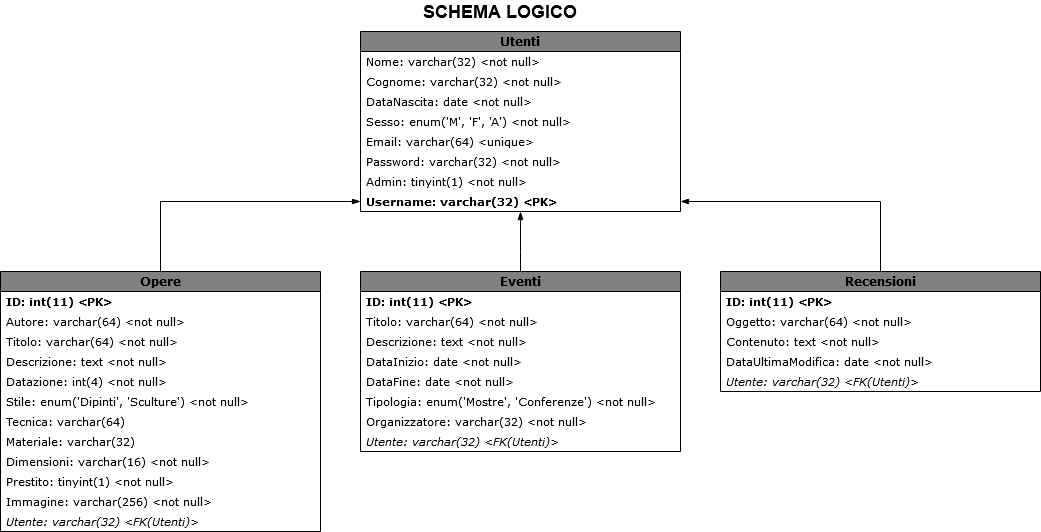
\includegraphics[width=\textwidth]{img/SchemaLogico}
	\captionof{figure}{Schema logico del database del museo \textit{TecArt}}
\end{center}

\subsection{Layout}
\label{progettazione-layout}
Per la scelta del design delle pagine, l'obiettivo è l'adattabilità al maggior numero possibile di dispositivi, indipendentemente dalle dimensioni dello schermo o dal supporto usato dall'utente. Si è puntato poi ad avere una struttura ordinata, leggera e di immediata comprensione e memorizzazione, al fine di rendere la navigazione semplice e intuitiva.
Per soddisfare queste esigenza è stato scelto il "layout a tre pannelli". Come da struttura standard, questo tipo di layout divide la schermata in tre settori: \textit{header} che deve contenere la rispota alla domanda "dove mi trovo?"; \textit{menu}, che deve contenere la rispota alla domanda "dove posso andare?"; \textit{content}, che deve contenere la rispota alla domanda "cosa c'è nella pagina?".
\begin{itemize}
	\item \textbf{\textit{Header}:} su \textit{desktop}, \textit{tablet} e \textit{mobile} occupa la fascia superiore della finestra ed è ampio quanto tutta la schermata. Riporta il nome del sito, il menu per l'accesso all'aera personale e la barra di ricerca. Nella parte più bassa contiene il \textit{breadcrumb}, che indica il percorso fatto dal visitatore all'interno del sito per arrivare alla pagina corrente. Per permettere agilmente all'utente di tornare alla pagine visitate in precedenza, il \textit{breadcrumb} si compone dei link delle pagine corrispondenti. 
	\item \textbf{\textit{Menu}}: riporta i link alle pagine principali del sito, contenenti tutte le informazioni rilevanti per la più ampia categoria di utenti.
	\item \textbf{\textit{Content}}: presenta il contenuto effettivo della pagina.
\end{itemize}
Nella parte più bassa della finestra, simmetricamente all'\textit{header}, si trova il \textit{footer}, che riporta le immagini certificanti la validazione, alcuni dettagli didattici e gli autori del sito. \\\\

In base alle dimensioni della finestra, questi elementi vengono visualizzati in modo diverso. A seguire, un esempio di design per i formati \textit{mobile}, \textit{tablet} e \textit{desktop}.

\begin{center}
	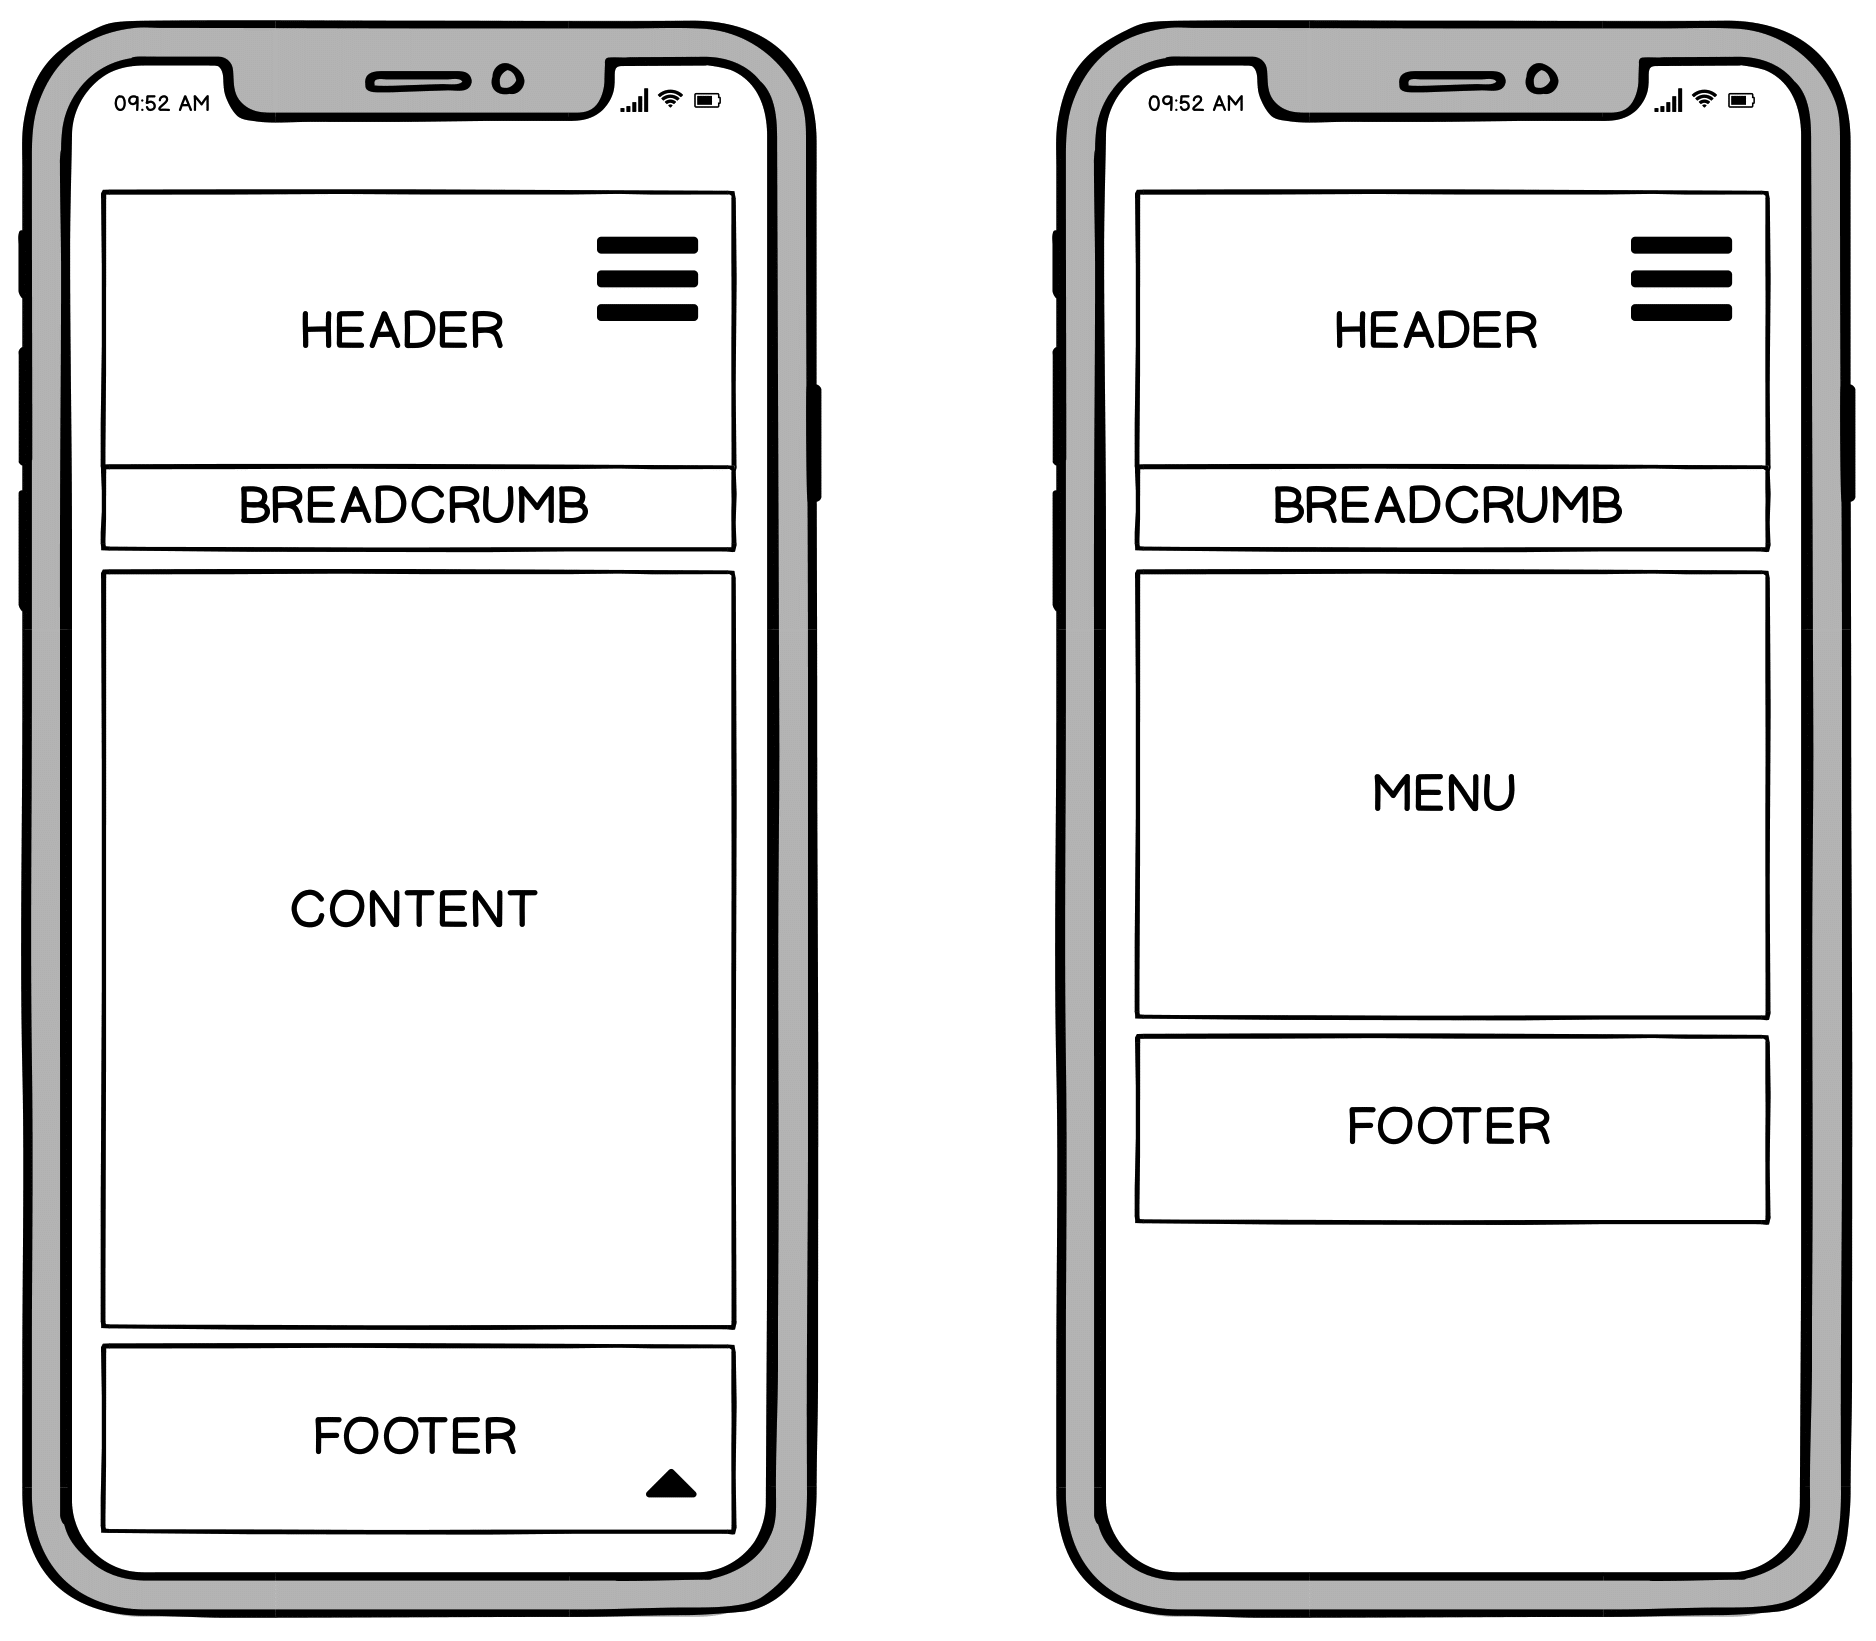
\includegraphics[scale=0.16]{img/Mobile}
	\captionof{figure}{Layout \textit{mobile} con \textit{menu} nascosto (a sinistra) e visibile (a destra)}
\end{center}

\begin{center}
	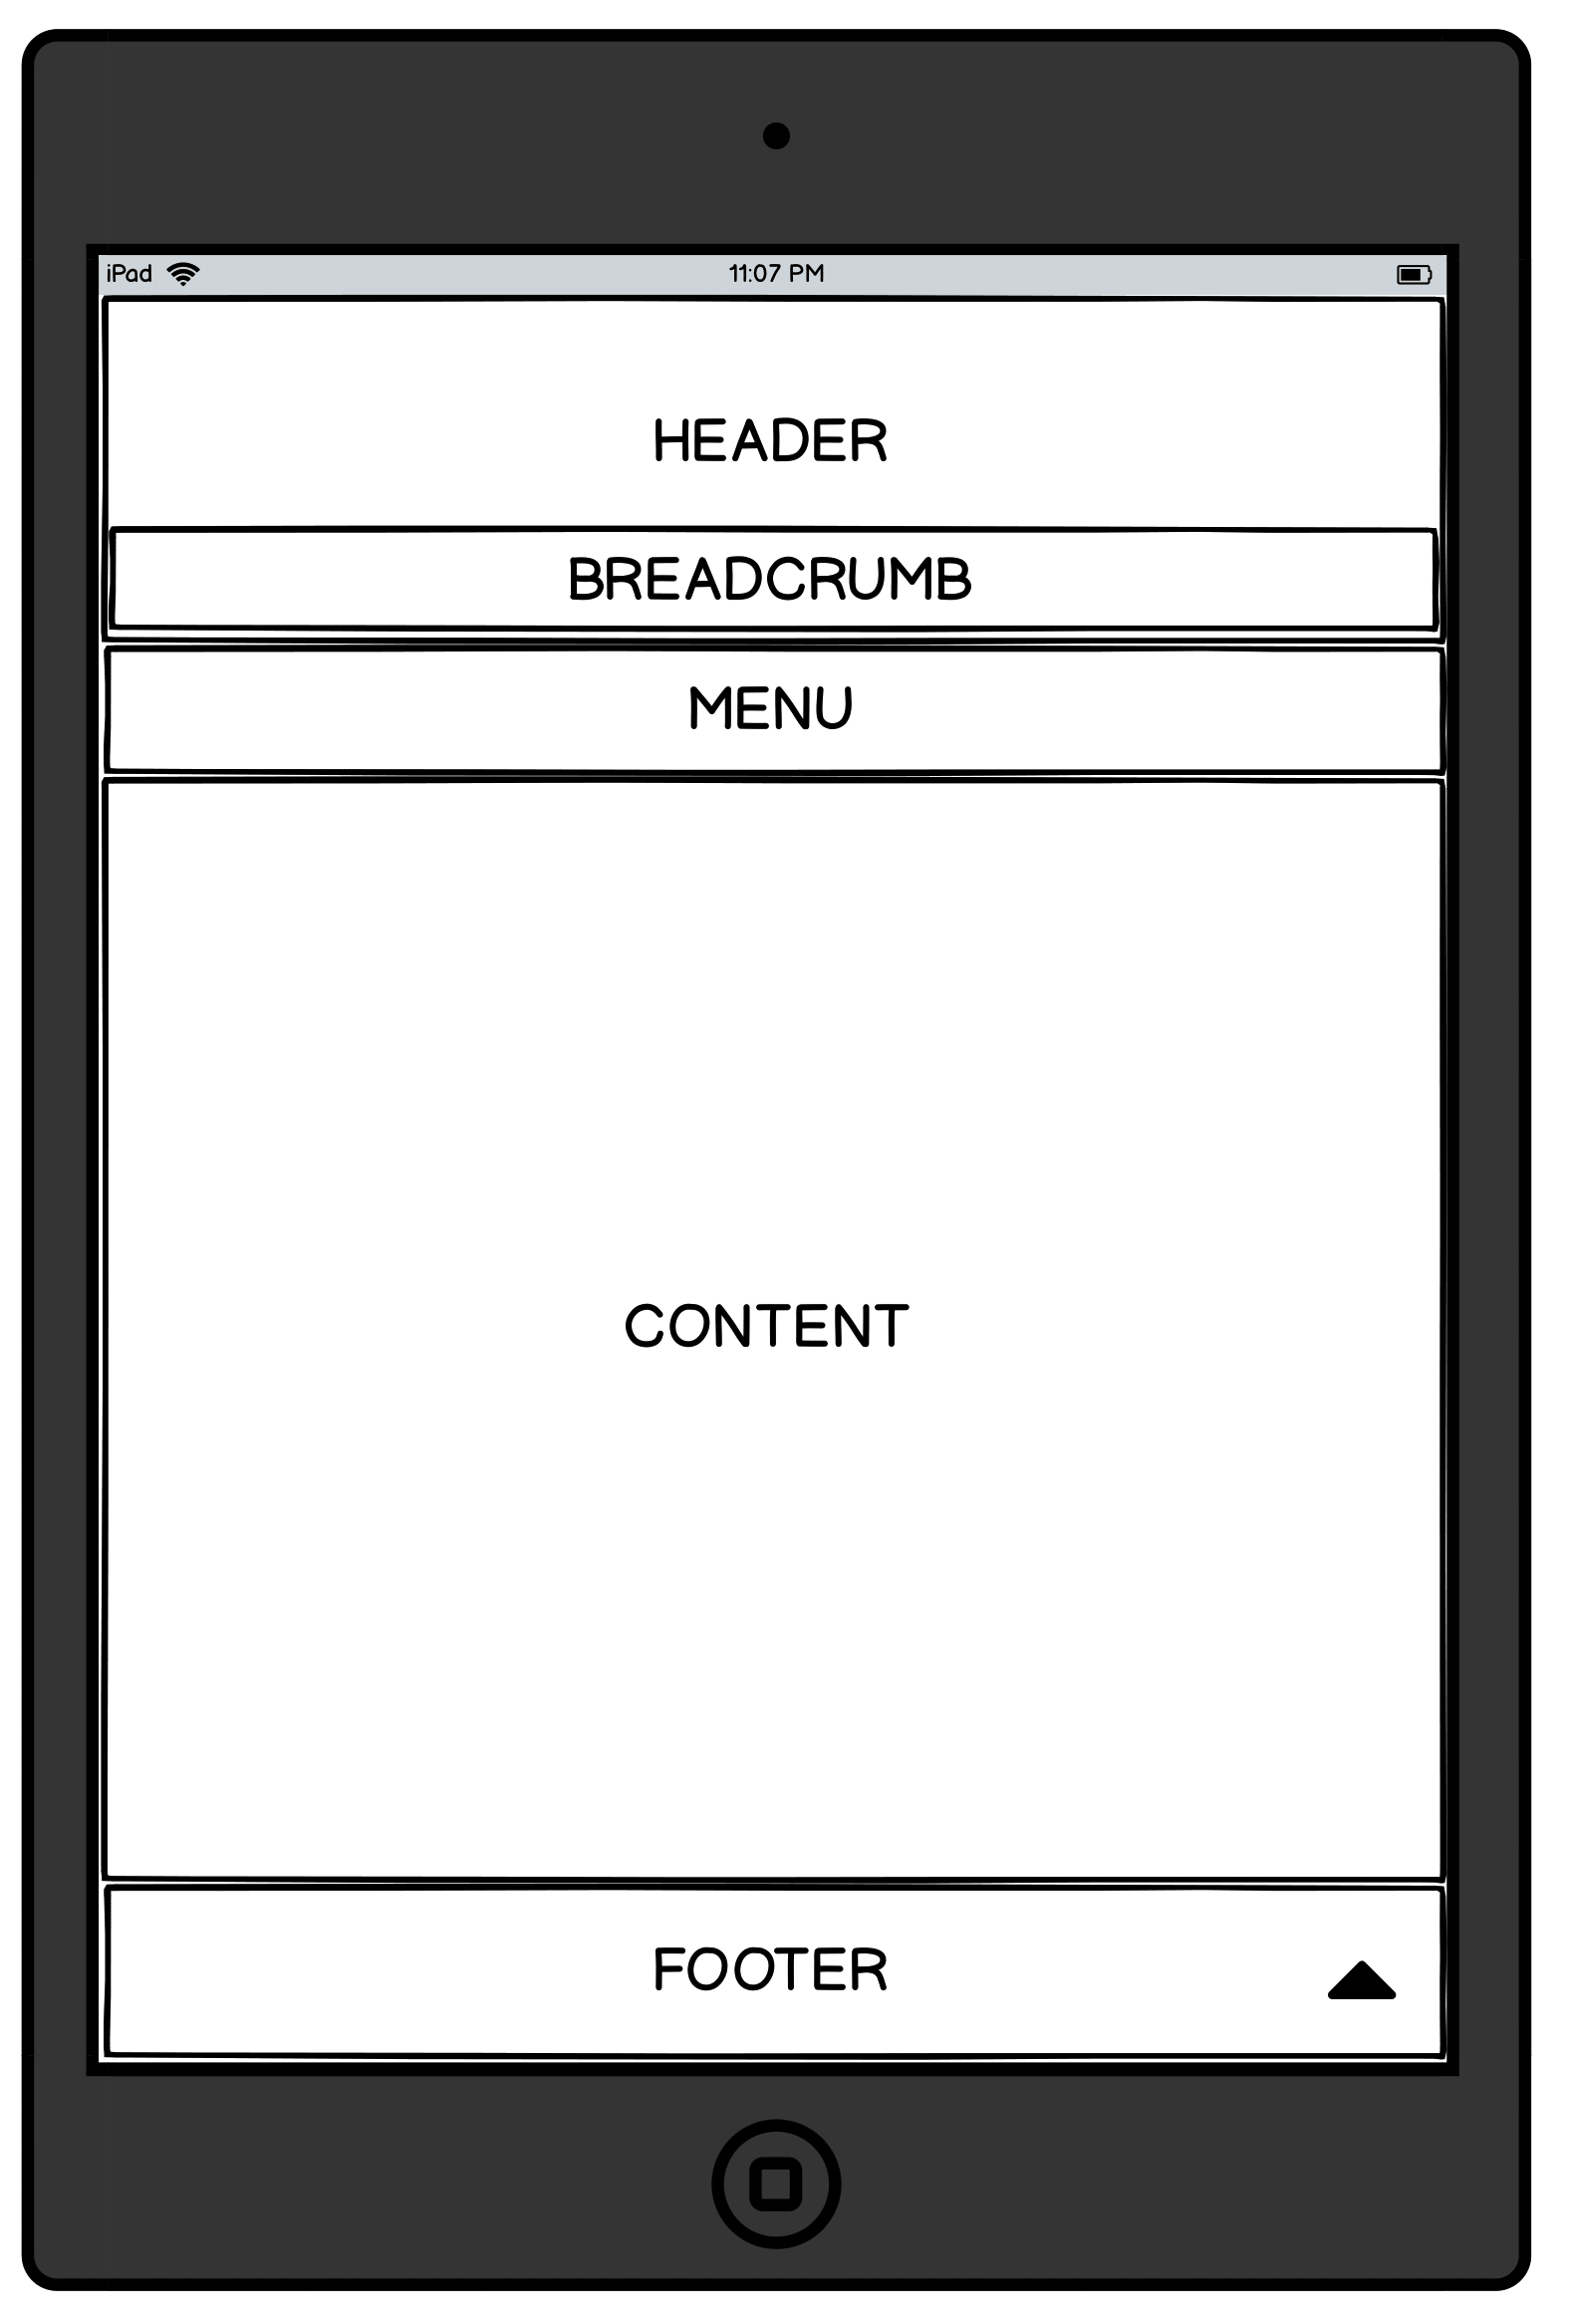
\includegraphics[scale=0.13]{img/Tablet}
	\captionof{figure}{Layout \textit{tablet}}
\end{center}

\begin{center}
	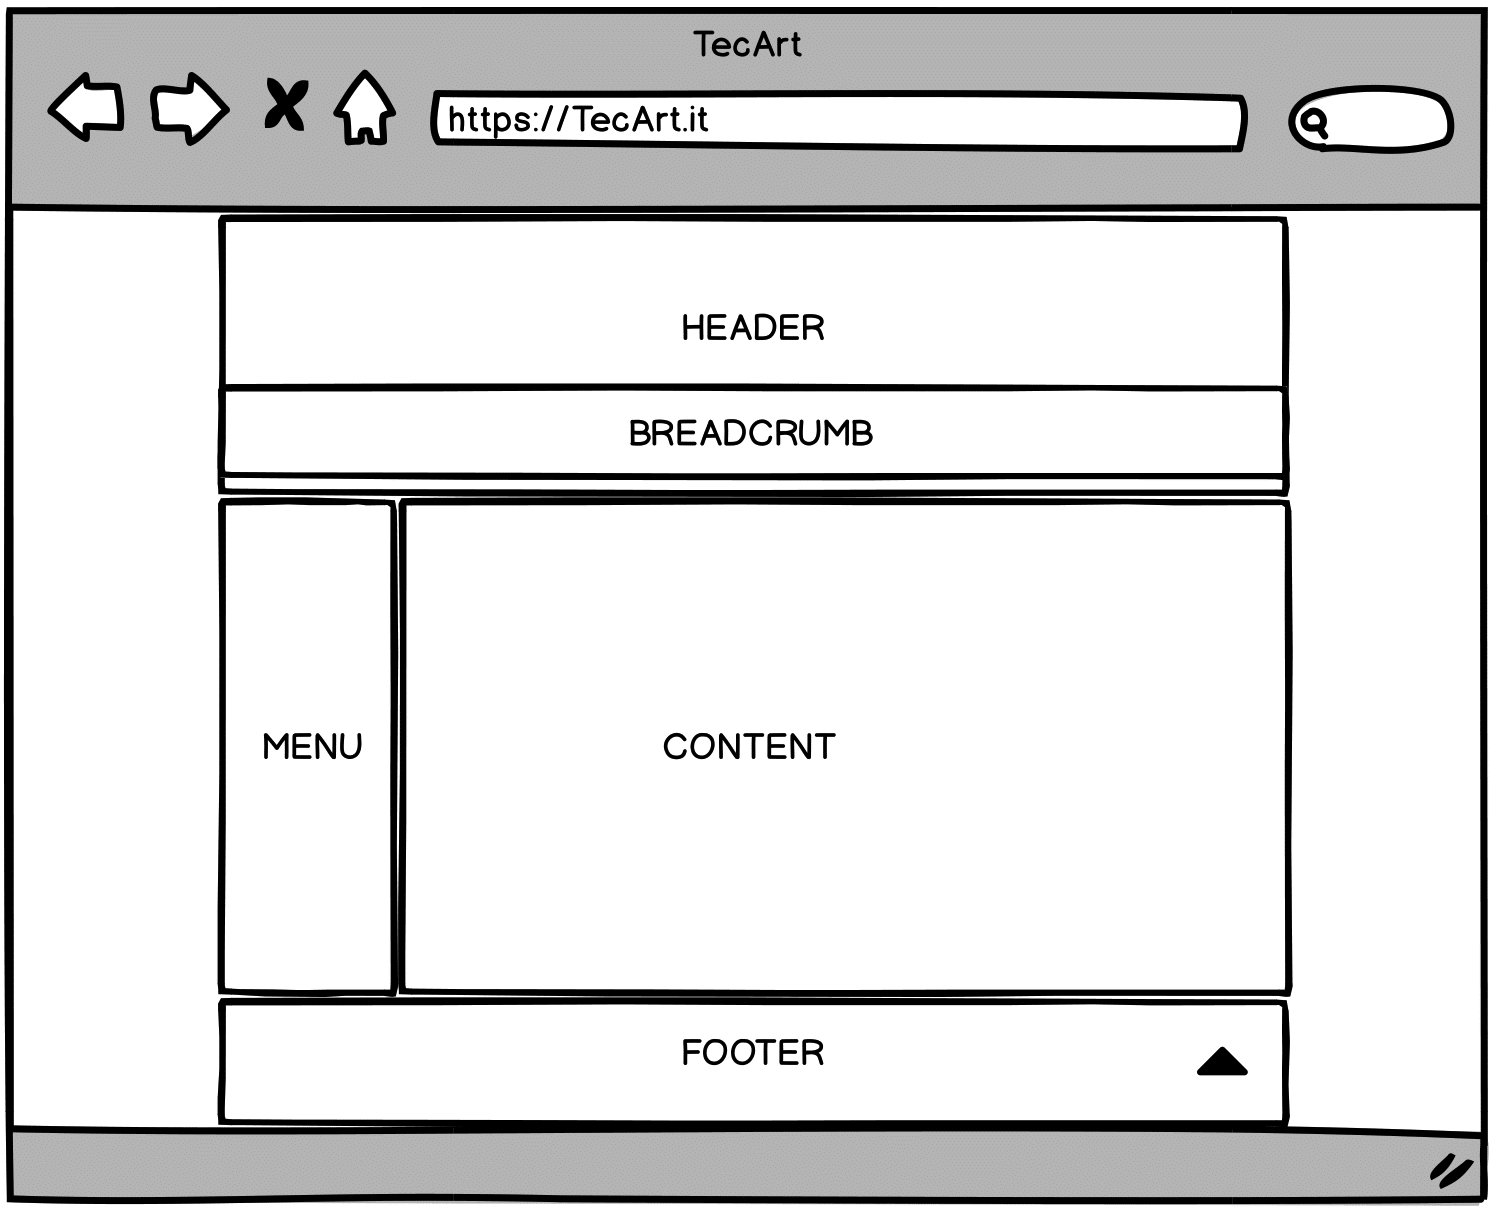
\includegraphics[width=\textwidth]{img/Desktop}
	\captionof{figure}{Layout \textit{desktop}}
\end{center}


\subsection{Accessibilità e usabilità}
\label{progettazione-accessibilità-usabilità}
Sin dalla fase di progettazione ogni aspetto del sito è stato pensato considerando le esigenze di tutte le possibili categorie di utenti. 


A questo scopo, nel rispetto delle specifiche di progetto, il gruppo si è ispirato ai seguenti principi:
\begin{itemize}
	\item \textbf{separazione tra struttura, presentazione e comportamento:} tutte le parti statiche delle pagine sono state implementate in XHTML Strict, la parte di presentazione grafica in CSS3, il comportamento con JavaScript, per i controlli dell'input lato \textit{client}, e PHP7, per i controlli dell'input lato server, la gestione dei contenuti e l'interazione con il database;
	
	\item \textbf{comprensibilità e navigabilità del sito:} l'organizzazione dei contenuti nelle varie pagine è stata pensata in modo che la struttura fosse coesa e comprensibile all'utente, e che la suddivisione aiutasse il visitatore a trovare tutte le informazioni desiderate nella pagina attesa;
	
	\item \textbf{contenuti equivalenti:} gli unici contenuti non testuali presenti nel sito sono le immagini, principalmente quelle delle opere esposte; per ogni figura è stato debitamente definito l'attributo \texttt{alt} del relativo tag HTML, in modo da fornire un'alternativa testuale coerente ed esplicativa del contenuto dell'immagine; in caso di immagini non semanticamente significative, esse sono inserite tramite CSS con la proprietà \texttt{background} (tecnica dell'\textit{image replacement});
	
	\item \textbf{scelta dello schema colori:} i colori del sito sono stati scelti in modo da non risultare di ostacolo alla consultazione per utenti ipovedenti o affetti da daltonismo; il software usato per i test è \textit{WebAIM} (\url{https://webaim.org/resources/contrastchecker/}); 
	
	\item \textbf{convenzioni colore per i link:} nel rispetto delle convenzioni più diffuse nei browser, i link risultano blu se mai visitati prima, altrimenti violetto; in ogni caso sono sottolineati. Unica eccezione a queste regole grafiche sono i button contenenti link: in questi casi non si è ritenuto necessario applicare le convenzioni sopra citate perché la forma stessa del button lo rende immediatamente riconoscibile come tale e perfettamente distinguibile dal resto del testo;
	
	\item \textbf{gestione delle peculiarità dei linguaggi naturali:} per facilitare la sintesi vocale, tutte le parole appartenenti a lingue diverse da quella indicata nell'attributo \texttt{xml:lang} di ogni pagina sono marcate opportunamente in modo da segnalare l'idioma di provenienza. Poichè il sito prevede la possibilità di inserimento di testo da parte degli utenti, autenticati o amministratori, i form di inserimento raccomandano di marcare eventuali termini stranieri con tag creati \textit{ad hoc}: in presenza di questi tag, tramite controlli PHP, al momento dell'inserimento del contenuto nella pagina del sito vengono inseriti i tag HTML corretti, con l'attributo \texttt{lang} impostato correttamente;
	
	\item \textbf{strutturazione delle pagine a prescindere dalla tecnologia in uso:} l'interfaccia utente è stata studiata in modo da essere intuitiva e di agile navigabilità anche per utenti con disabilità visive non totalmente invalidanti. Gli elementi grafici sono stati dimensionati in modo da non essere nè troppo grandi (caratteristica che li renderebbe inadatti alla fruizione tramite \textit{magnifier} o altri strumenti di ingrandimento) nè troppo piccoli (aspetto che renderebbe difficile la navigazione a chiunque non avesse una vista ottima). Si è avuta cura che le scelte di progettazione e grafiche tenessero fossero compatibili anche con le versioni più vecchie dei vari browser, e quando ciò non è stato possibile si è cercato di garantire il più possibile la traformazione elegante (vedi §\ref{implementazione});
	
	\item \textbf{adozione della tecnologia \textit{WAI ARIA}:} per agevolare la lettura da parte di \textit{screen reader}, sono stati aggiunti gli attributi \texttt{aria-label}  ad alcuni elementi HTML , in modo che ad ognuno fosse associato un testo contenente la funzionalità del campo evidenziato, e \texttt{aria-required=true} sui campi obbligatori dei form.
	
	\item \textbf{guida alla navigazione:}
	\begin{itemize}
		\item \textbf{breadcrumb}: l'utente ha sempre a disposizione la sequenza ordinata delle pagine visitate per arrivare a quella corrente, così da evitare disorientamento;
		\item \textbf{tabindex:} questo attributo non è stato fissato a valori positivi poiché l'ordine del DOM corrispondeva già a quello desiderato per la navigazione. L'unico caso in cui è stato necessario definirlo è stato il menu \textit{ad hamburger} nella grafica \textit{mobile}: per renderlo \textit{focusable} nella navigazione tramite tab, il suo tabindex è stato posto a 0;
		\item \textbf{link \texttt{torna su}:} per raggiungere rapidamente l'\textit{header} della pagina (o comunque la sua parte iniziale), senza dover fare scroll verso l'alto;
		\item \textbf{link \texttt{salta al...}:} per gli utenti che non possono usare puntatore o mouse per arrivare rapidamente al contenuto desiderato, sono stati predisposti dei link interni alle pagine per raggiungere direttamente alcuni punti significativi del contenuto (per esempio, evitare tutto lo scorrimento del menu e passare direttamente al corpo della pagina).
	\end{itemize}
\end{itemize}
